% Krasner's lemma: beta closer to alpha than any conjugate of alpha (generated by a script).
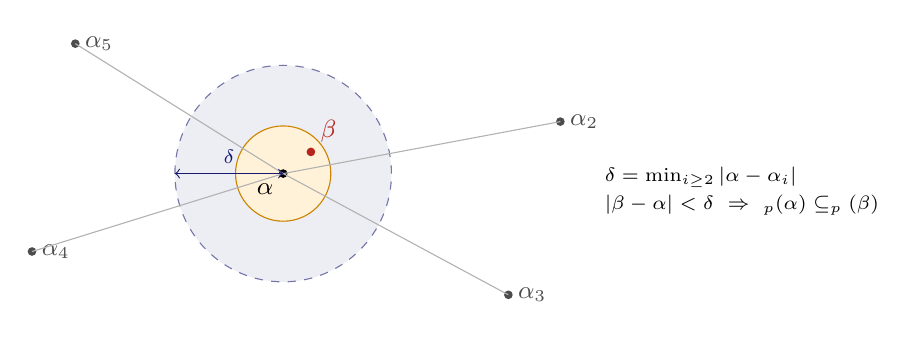
\begin{tikzpicture}[scale=1.1]
\fill[MidnightBlue!8] (0,0) circle (1.25);
\draw[MidnightBlue!60,dashed] (0,0) circle (1.25);
\fill[Orange!15] (0,0) circle (0.55);
\draw[Orange!80!black] (0,0) circle (0.55);
\fill[black] (0,0) circle (0.05) node[below left,font=\small]{$\alpha$};
\fill[BrickRed] (0.32,0.25) circle (0.05) node[above right,font=\small,BrickRed]{$\beta$};
\fill[black!70] (3.20,0.60) circle (0.05) node[right,font=\small]{$\alpha_{2}$};
\draw[black!30] (0,0)--(3.20,0.60);
\fill[black!70] (2.60,-1.40) circle (0.05) node[right,font=\small]{$\alpha_{3}$};
\draw[black!30] (0,0)--(2.60,-1.40);
\fill[black!70] (-2.90,-0.90) circle (0.05) node[right,font=\small]{$\alpha_{4}$};
\draw[black!30] (0,0)--(-2.90,-0.90);
\fill[black!70] (-2.40,1.50) circle (0.05) node[right,font=\small]{$\alpha_{5}$};
\draw[black!30] (0,0)--(-2.40,1.50);
\draw[<->,MidnightBlue] (0,0)--(-1.25,0) node[midway,above,font=\scriptsize]{$\delta$};
\node[font=\scriptsize,align=left,anchor=west] at (3.6,-0.2) {$\delta=\min_{i\ge2}|\alpha-\alpha_i|$\\[2pt] $|\beta-\alpha|<\delta\ \Rightarrow\ \Q_p(\alpha)\subseteq\Q_p(\beta)$};
\end{tikzpicture}
